\section{$k$-clique Problem}

%!% rozmyslet a překopat nach einem Muster:

$k$-clique Problem belongs to $\NPC$ problems, its task is to decide whether there exists a clique with $k$ vertices in given graph $G$. Note that there exists a $k$-clique in $G$ iff there exists a $k$-independent set in $\overline{G}$ iff there exists an $(n-k)$-vertex cover of $\overline{G}$. Thus we can assume $k \leq \frac{n}{2}$ because those verification algorithms would be very similar.

From technical reasons we need $k$ to be even in all following examples; reduction from odd numbers will be solved in every single example.

Here if $k$ is odd, we add another vertex connected to every original vertex resulting in $G'$. Then existence of $(k+1)$-clique in $G'$ is equivalent to existence of $k$-clique in $G$. In following example in Figure \ref{fig:k-clique} we take $k$ even.

% reduction from SAT (wiki)

% vocad

\subsection*{Set of tiles}

\begin{description}
	\item[Bottom tiles] There are tiles with $2l-2$ and $2l$ $(0 < l \leq \frac{k}{2})$ in this order on the bottom sides and with all possible numerically ordered\footnote{Later we will order by color.} pairs of connected numbers\footnote{Note that this restriction does not reduce the set of candidate $k$-cliques.} from $1$ to $n$ having $(k-2l+2)$-th and $(k-2l+1)$-th color, respectively, on the top sides. %!% check: $\frac{kn^2}{4}$ tile types were required.
	\item[Bottom corner tiles] Both corner tiles are connected on the bottom by the lowest and the highest non-colored number, respectively, and have their special glue (\# can be viewed as $-\infty$ with respect to used ordering and * as $+\infty$) on the top. $2$ tile types were required.
	\item[Inner tiles] These tiles are responsible for ordering by color during which they verify existence of {\em every} edge ...% in similar manner to previous problems.
	% Because the first line contains them in reverse order they will meet each other. $k^2 n^2$ tile types were required. % $k^2 \cdot 2#E $
	\item[Border tiles] These tiles are exactly the same like for 3-coloring.
	\item[Verification tiles] As soon as the most left color reaches sharp and the most right color reaches asterisk, verification is triggered in similar manner to 3-coloring. $kn$ tile types were required.
	\item[DONE tile] This is exactly the same like 3-coloring. $1$ tile type was required.
\end{description}
Summed up, this DNA algorithm requires $k^2 n^2$ tile types. Binding complexity is $1\nicefrac{1}{4}\,k^2$. Glue complexity is ... % $k^2 \cdot 2#E $

\begin{figure}[H]
\begin{center}
	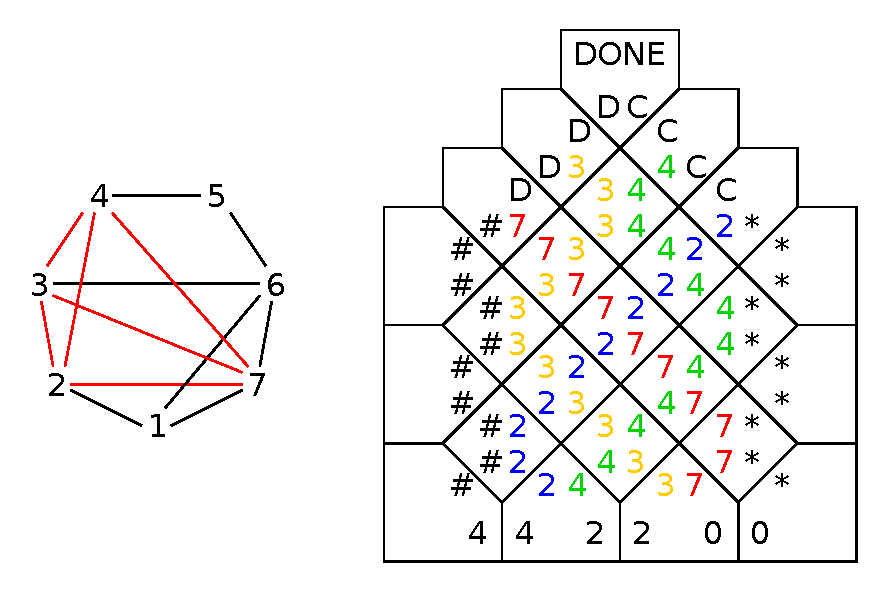
\includegraphics[scale=0.75]{./figures/k-clique/k-clique.pdf}
	\caption{$k$-clique computation. Color order is defined by their wavelength.}
	\label{fig:k-clique}
\end{center}
\end{figure}

